\section{Le développement de \textsc{Sigma}}

\subsection{Création de la structure de la base de données}

Avant de commencer le développement, Clément \textsc{Martaille} et Alexandre \textsc{Meunier} commencèrent par concevoir la base de données.
L'idée était de créer la structure générale de la base de données afin de visualiser plus facilement l'ensemble du projet et de pouvoir déterminer les priorités dans le développement.
En effet, une fois la structure globale de la base construite, il est possible de voir les tables de la base qui seront utilisées par le plus d'applications et modules différents.
Ce sont ces applications qui devront être développées en premières et pour lesquelles il faudra porter une attention particulière à ce qu'elles soient simples et stables, étant donné qu'elles serviront de base au reste du projet.

Une fois la structure de la base de données terminée, il fut déterminé que le premier module à développer serait celui de la gestion des clients, le CRM.
Comme dit auparavant, ce choix fut pris en raison du fait que la gestion des clients, de leurs adresses, des contacts, etc., représente le coeur du projet.

\subsection{Application de la méthode itérative incrémentale}

Pour chaque application de \textsc{Sigma}, nous appliquons la même méthode de travail, sa mise en pratique respecte toujours les mêmes grandes étapes.

\FloatBarrier
\begin{figure}[h!]
    \begin{center}
        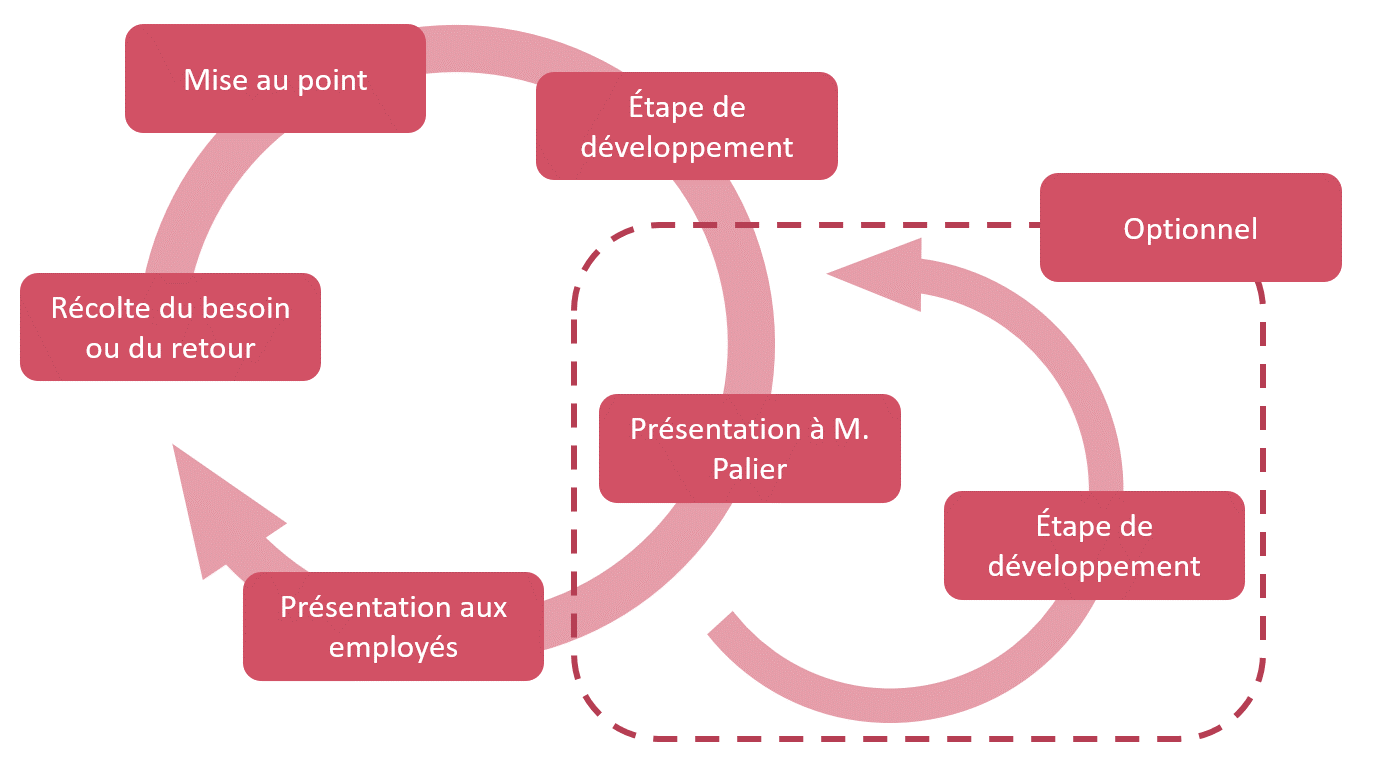
\includegraphics[width = 0.9\textwidth]{cycle_dev}
    \end{center}
    \caption{Cycle de développement}
    \label{figure:cycle_dev}
\end{figure}
\FloatBarrier

La première étape est la récolte du besoin.
Dans un premier temps M. \textsc{Palier}, s'entretenait avec les futurs utilisateurs pour recueillir leurs besoins et me les retransmettre de manière claire et plus adaptée pour le développement.
Au cours de l'avancement de mon apprentissage, il me laissa plus de responsabilités vis-à-vis de la récolte et de l'analyse des besoins.
Désormais, M. \textsc{Palier} suit toujours l'avancement de mon travail, mais il me laisse m'entretenir avec les employés et responsables de service lorsque j'en ai besoin.

Une fois le besoin éclairci, si nécessaire, je m'entretiens avec M. \textsc{Palier} pour discuter des potentielles modifications à apporter à la base de données et également des modifications et ajouts nécessaires au niveau des applications de \textsc{Sigma}.
Cette mise au point permet de s'assurer que le développement à prévoir n'entre pas en conflit avec un autre développement passé, en cours, ou futur.

Suite à cette mise au point, je commence les modifications de la base de données et la création des mock-ups des différentes fenêtres à développer.
Ces mock-ups permettent de présenter les avancées aux futurs utilisateurs en leur expliquant de manière concrète les fonctionnalités imaginées.
Les futurs utilisateurs peuvent alors se faire une idée claire du résultat futur et nous faire part de leurs retours.
Au début de mon apprentissage je présentais constamment les mock-ups à M. \textsc{Palier} pour avoir son retour avant de les présenter aux employés, mais désormais il est courant que je les présente directement aux utilisateurs finaux.
Cela permet d'économiser du temps, ce qui est d'autant plus vrai maintenant que celui-ci n'est plus présent dans les locaux de \textsc{Disa}.

Une fois les maquettes présentées, nous utilisons le retour afin de les améliorer et de commencer à implémenter les fonctionnalités imaginées.
C'est un cycle de développement qui se répète jusqu'à l'obtention d'un produit final satisfaisant pour les utilisateurs comme pour le développeur.
Ce cycle est basé sur le retour des utilisateurs ce qui permet de s'assurer un développement dans la bonne direction et ainsi garantir un produit adapté à leurs besoins.

\subsection{Mise en production progressive de \textsc{Sigma}}

La mise en production de \textsc{Sigma} s'est effectuée très progressivement et commença dès le début de l'année 2018.

Dans un premier temps, nous avons installé l'application sur les postes des responsables projets et nous les avons formés à l'utilisation de l'outil d'édition de devis.
Cette première étape de mise en production nous a permis de commencer la formation de certains employés et surtout d'obtenir des retours concrets, et ainsi, de corriger de nombreux défauts.

Nous avons ensuite suivi cette même méthodologie pour la suite de la mise en production.
Cela nous a permis de former les employés à l'utilisation des parties de \textsc{Sigma} qui leur sont dédiés, le tout sans être débordés.
Un gros avantage avec cette méthode est que les retours des utilisateurs se font progressivement, ce qui nous laisse le temps d'apporter des modifications et de nous assurer que celles-ci conviennent pour tous les utilisateurs.

À l'heure actuelle, tous les employés de \textsc{Disa} utilisent \textsc{Sigma} et ils sont formés à l'utilisation de leurs applications dédiées.
Nous nous concentrons sur la résolution des bugs qui se font de moins en moins présents, et surtout sur l'amélioration de certaines fonctionnalités sur la demande des utilisateurs.
Il y a encore plusieurs applications à créer sous \textsc{Sigma} afin de pouvoir remplacer complètement ASAP et \textsc{Disanet}.
